% \documentclass[crop,convert={density=600,outext=.png}]{standalone}% 'crop' is the default for v1.0, before it was 'preview'
\documentclass[border=4mm,convert={density=400,size=600,outext=.png}]{standalone}

% run with pdflatex --shell-escape 
% orto get the png image
% check there are permissions in the new Ubuntu (2023+):
% 	https://stackoverflow.com/a/59193253



\usepackage{tikz}
\usetikzlibrary{shapes,arrows,snakes}
\usetikzlibrary{backgrounds}

% We need layers to draw the block diagram
\pgfdeclarelayer{background}
\pgfdeclarelayer{foreground}
\pgfsetlayers{background,main,foreground}

\usepackage{amsmath,amssymb}

\usetikzlibrary{calc}



\begin{document}

% Define box and box title style
\tikzstyle{mybox} = [draw=red, fill=blue!20, very thick, rectangle, rounded corners, inner sep=5pt, inner ysep=5pt]
\tikzstyle{fancytitle} =[fill=red, text=white]

%% ARROWS
\tikzstyle{goal} =[draw, ->]
\tikzstyle{report} =[draw, dashed, ->]
\tikzstyle{talk} =[draw, dotted, <->,very thick]

\definecolor{blueprintcolor}{RGB}{20,20,100}

% The light color
\colorlet{light}{white!90!blueprintcolor}

% The background color
\colorlet{background}{black!10}

% \module{name}{title}{text}{file}
\newcommand{\module}[5]{
	\node [mybox,text width=0.20\textwidth] [#2] (#1){%
		\smallskip
		\begin{center}
			#4 \\[1ex]
			#5
		\end{center}
	};
	\node[fancytitle, right=10pt] at (#1.north west) {#3};
}
\def\blockdist{2.3}
\def\edgedist{2.5}

\begin{tikzpicture}[node distance=4cm
		% ,show background rectangle,
		% background rectangle/.style={fill=background}
	]
	\module{main}{fill=red!30}{Main Cycle}{Top-level Execution Cycle}{indigolog.pl}


	\module{envman}{left of=main,xshift=-3cm,text width=4cm}{Environment
		Manager}{Middlware devices and executor (actions + sensing + exog events)}{env\_man.pl}

	\path[goal] ($(main.west)-(0,0.5)$) -- node[below]
	{\begin{tabular}{c}
			\texttt{execute\_action/4}
		\end{tabular}
	}
	($(envman.east)-(0, 0.5)$);

	\path [report] (envman.east) -- node [above,sloped]
	{\begin{tabular}{c}
			asserts exog actions \\
			\texttt{pending/1}
		\end{tabular}
	}
	(main.west);


	\module{trans}{right of=main,xshift=2cm}{Trans}
	{Single step semantics}{transfinal.pl}

	\module{eval}{below of=trans,yshift=-1cm}{Projector}
	{Evaluates formulas}{eval.pl}



	\path [goal] (main) --
	node [above]  {query transition}
	node [below]  {\begin{tabular}{c}
			\texttt{trans/4} \\
			\texttt{final/2}
		\end{tabular}
	}
	(trans);

	\path [goal] (trans) -- node[xshift=0.8cm]   {\texttt{holds/2}} ($(eval.north)+(0,0.3)$);


	\path [goal] (main) --
	node [above,sloped]
	{\begin{tabular}{c}
			\texttt{handle\_sensing/4}
		\end{tabular}}
	node [below,sloped]
	{\begin{tabular}{c}
			\texttt{progress\_db/2}
		\end{tabular}}
	(eval);

	%%%%% DOMAIN APPLICATION
	\module{domexec}{below of=envman,yshift=-1cm}{Application}
	{Execution information}{main.pl}

	\module{axioms}{right of=domexec,xshift=0.3cm}{Axioms}
	{Domain axiomatization}{domain.pl}

	\module{program}{above right of=axioms,shift={(0.3cm,-1.6cm)}}{Programs}
	{High-level programs}{domain.pl}

	\path [goal] (envman.south) -- node
	[xshift=1.7cm]
	{\begin{tabular}{c}
			\texttt{load\_devices/2}    \\
			\texttt{how\_to\_execute/3} \\
			\texttt{translate\_exog/2}  \\
			\texttt{translate\_sensing/3}
		\end{tabular}}
	($(domexec.north)+(0,0.3)$);

	% main file loads axioms and program
	% \path [goal] (axioms) -- (domexec);
	% \path [goal] (program) -- (domexec);

	\path [goal] (eval) -- (axioms.east);

	\path [goal] (trans.south west) -- (program.east);

	%%%%%%% DEVICES
	\module{webdev}{above of=envman,shift={(0cm,1cm)}}{Web Device}
	{Manager for WWW}{dev\_www.pl}
	\module{er1dev}{right of=webdev}{ER1 Device}
	{Manager for ER1 robot}{dev\_er1.pl}
	\module{rcxdev}{right of=er1dev}{RCX Device}
	{Manager for Lego RCX}{dev\_rcx.pl}
	\module{simdev}{right of=rcxdev}{SIM Device}
	{Simulator in terminal}{dev\_sim.pl}

	\path [talk] (envman.north)+(0,0.5) -- node[sloped,above] {} (webdev.south);
	\path [talk] (envman.north)+(0,0.5) -- node[sloped,above] {} (er1dev.south);
	\path [talk] (envman.north)+(0,0.5) -- node[sloped,above] {} (rcxdev.south);
	\path [talk] (envman.north)+(0,0.5) -- node
		{\Large TCP/IP Socket Communication} (simdev.south);


	%  \node [above of=webdev] (web) {\includegraphics[height=1.5cm]{img/network}};
	\node [above of=webdev] (web) {
\includegraphics[height=1.5cm]{img/kinternet}};
	\path [draw,<->] (webdev.north)+(0,.3) -- (web);

	%  \node [above of=er1dev] (er1) {\includegraphics[height=1.5cm]{img/robot1}};
	\node [above of=er1dev] (er1) {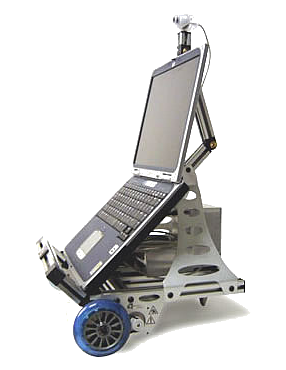
\includegraphics[height=2.0cm]{img/ER1-robot}};
	\path [draw,<->] (er1dev.north)+(0,.3) -- (er1);

	\node [above of=rcxdev] (rcx) {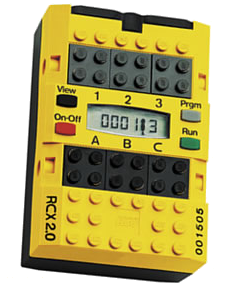
\includegraphics[height=1.7cm]{img/rcx}};
	\path [draw,<->] (rcxdev.north)+(0,.3) -- (rcx);

	%  \node [above of=simdev] (sim) {\includegraphics[height=1.5cm]{img/xterm}};
	\node [above of=simdev] (sim) {
\includegraphics[height=1.5cm]{img/konsole}};
	\path [draw,<->] (simdev.north)+(0,.3) -- (sim);

	\begin{pgfonlayer}{background}
		% Compute a few helper coordinates
		\path (envman.west |- envman.north)+(-0.2,0.5) node (a) {};
		\path (eval.south -| eval.east)+(+0.2,-0.4) node (b) {};
		\path[fill=yellow!20,rounded corners, draw=black!50, dashed]
		(a) rectangle (b);


		\path (program.east |- program.north)+(+0.2,0.4) node (a) {};
		\path (domexec.south -| domexec.west)+(-0.2,-0.2) node (b) {};
		\path[fill=green!20,rounded corners, draw=black!50, dashed]
		(a) rectangle (b);

		\path (envman.west |- envman.north)+(-0.1,0.4) node (a) {};
		\path (main.south -| main.east)+(+0.2,-0.4) node (b) {};
		\path[fill=red!20,rounded corners, draw=black!50, dashed]
		(a) rectangle (b);
	\end{pgfonlayer}
\end{tikzpicture}

\end{document}
